\documentclass[aspectratio=169]{beamer}
% Add slides directory to search path for Dartmouth theme
\makeatletter
\def\input@path{{../}}
\makeatother
\usetheme{Dartmouth}
\usepackage{booktabs}
\usepackage{listings}
\usepackage{tikz}
\usetikzlibrary{arrows.meta,positioning,shapes,decorations.pathreplacing}
\usepackage{hyperref}
\usepackage{xcolor}
\usepackage{graphicx}
\usepackage{fontspec}
\usepackage{tcolorbox}
\usepackage{amsmath}
\usepackage{amssymb}

% Color scheme
\definecolor{darkblue}{RGB}{0,82,155}
\definecolor{lightblue}{RGB}{100,181,246}
\definecolor{darkgreen}{RGB}{46,125,50}
\definecolor{orange}{RGB}{255,152,0}
\definecolor{purple}{RGB}{142,36,170}
\definecolor{thinkbox}{RGB}{255,245,220}
\definecolor{discussbox}{RGB}{230,240,255}

\setbeamercolor{frametitle}{bg=darkblue}
\setbeamercolor{progress bar}{fg=lightblue,bg=lightblue!30}

% Code listing settings
\lstset{
    basicstyle=\ttfamily\small,
    breaklines=true,
    frame=single,
    backgroundcolor=\color{gray!10},
    keywordstyle=\color{darkblue}\bfseries,
    commentstyle=\color{darkgreen}\itshape,
    stringstyle=\color{orange},
    showstringspaces=false,
    language=Python
}

% Custom boxes
\newtcolorbox{thinkaboutit}{
    colback=thinkbox,
    colframe=orange,
    title=💭 Think about it!,
    fonttitle=\bfseries
}

\newtcolorbox{discussion}{
    colback=discussbox,
    colframe=blue,
    title=💬 Discussion,
    fonttitle=\bfseries
}

\title{Week 7: Models of Conversation}
\subtitle{Pragmatics, Dialogue, and Thought Trajectories 💬}
\author{Models of Language and Conversation}
\institute{Dr. Jeremy R. Manning}
\date{}

\begin{document}

% Title slide
\begin{frame}
    \titlepage
\end{frame}

% Table of contents
\begin{frame}{Today's Journey 🗺️}
    \tableofcontents
\end{frame}

\section{What is Language Used For?}

\begin{frame}[shrink=10]{What is Language Used For? 🎭}
\small
    \begin{discussion}
        Why do we use language? What is its \textit{purpose}?
    \end{discussion}

    \vspace{0.3cm}

    \begin{columns}[T]
        \begin{column}{0.5\textwidth}
            \textbf{Traditional view:}
            \begin{itemize}\setlength{\itemsep}{0pt}
                \item 📢 Transmitting information
                \item 🧠 Expressing thoughts
                \item 📝 Describing the world
                \item 🎓 Teaching/learning
            \end{itemize}
        \end{column}

        \begin{column}{0.5\textwidth}
            \textbf{Pragmatic view:}
            \begin{itemize}\setlength{\itemsep}{0pt}
                \item 🤝 Coordinating actions
                \item 🎯 Achieving goals
                \item 👥 Building relationships
                \item 🌐 Creating shared reality
            \end{itemize}
        \end{column}
    \end{columns}

    \vspace{0.3cm}

    \begin{alertblock}{Key Insight}
        Language is fundamentally a \textbf{tool for action}, not just description!
    \end{alertblock}
\end{frame}

\begin{frame}{Language as Action 🎬}
\small
    \textbf{Speech Acts (Austin, 1962; Searle, 1969):}

    \vspace{0.3cm}

    \begin{enumerate}\setlength{\itemsep}{0pt}
        \item \textbf{Assertives}: Committing to truth \\
        \textit{"It's raining outside."}

        \item \textbf{Directives}: Getting someone to do something \\
        \textit{"Please close the window."}

        \item \textbf{Commissives}: Committing to future action \\
        \textit{"I promise to help you."}

        \item \textbf{Expressives}: Expressing psychological states \\
        \textit{"I'm sorry for being late."}

        \item \textbf{Declarations}: Changing the world by saying so \\
        \textit{"I now pronounce you married."}
    \end{enumerate}

    \vspace{0.3cm}

    \begin{thinkaboutit}
        When you say "It's cold in here," are you just describing temperature, or asking someone to close a window?
    \end{thinkaboutit}
\end{frame}

\begin{frame}[shrink=10]{Beyond Literal Meaning 🧩}
\small
    \textbf{Same words, different meanings in context:}

    \vspace{0.3cm}

    \begin{block}{Example 1: "Can you pass the salt?"}
        \begin{itemize}\setlength{\itemsep}{0pt}
            \item \textbf{Literal meaning}: Question about ability
            \item \textbf{Pragmatic meaning}: Request for action
            \item Nobody answers: "Yes, I can" and then does nothing!
        \end{itemize}
    \end{block}

    \vspace{0.3cm}

    \begin{block}{Example 2: "It's getting late."}
        \begin{itemize}\setlength{\itemsep}{0pt}
            \item At dinner party $\rightarrow$ "I should leave"
            \item To children $\rightarrow$ "Go to bed"
            \item To colleague $\rightarrow$ "Let's finish this meeting"
            \item Context determines interpretation!
        \end{itemize}
    \end{block}

    \vspace{0.3cm}

    \textbf{This is \textit{pragmatics}}: How context shapes meaning beyond literal words
\end{frame}

\section{Pragmatics and Dialogue}

\begin{frame}{Pragmatics: The Study of Language in Use 📚}
\small
    \begin{block}{Definition}
        \textbf{Pragmatics} is the study of how context influences language interpretation and use.
    \end{block}

    \vspace{0.3cm}

    \textbf{Key concepts:}
    \begin{itemize}\setlength{\itemsep}{0pt}
        \item \textbf{Context}: Physical, social, temporal, cultural
        \item \textbf{Implicature}: Implied meaning beyond literal words (Grice, 1975)
        \item \textbf{Common ground}: Shared knowledge between speakers
        \item \textbf{Grounding}: Process of establishing mutual understanding
        \item \textbf{Alignment}: Speakers coordinating their representations
    \end{itemize}

    \vspace{0.3cm}

    \begin{alertblock}{Why This Matters for LLMs}
        Modern language models excel at syntax and semantics, but struggle with pragmatics!
    \end{alertblock}
\end{frame}

\begin{frame}{Common Ground: Shared Knowledge 🤝}
\small
    \begin{block}{Clark \& Brennan (1991)}
        \textit{Grounding in Communication}: Communication is a \textbf{collaborative activity} requiring common ground.
    \end{block}

    \vspace{0.3cm}

    \textbf{What is common ground?}
    \begin{itemize}\setlength{\itemsep}{0pt}
        \item Mutual knowledge, beliefs, and assumptions
        \item Shared perceptual experience
        \item Cultural knowledge
        \item Previous conversation history
        \item Physical co-presence
    \end{itemize}

    \vspace{0.3cm}

    \begin{columns}[T]
        \begin{column}{0.5\textwidth}
            \textbf{Example with common ground:}

            \textit{A: "Did you see the game?"}

            \textit{B: "Yeah, incredible comeback!"}
        \end{column}

        \begin{column}{0.5\textwidth}
            \textbf{Without common ground:}

            \textit{A: "Did you see the game?"}

            \textit{B: "What game?"}
        \end{column}
    \end{columns}
\end{frame}

\begin{frame}[shrink=5]{Visualizing Common Ground 🎯}
    \begin{center}
        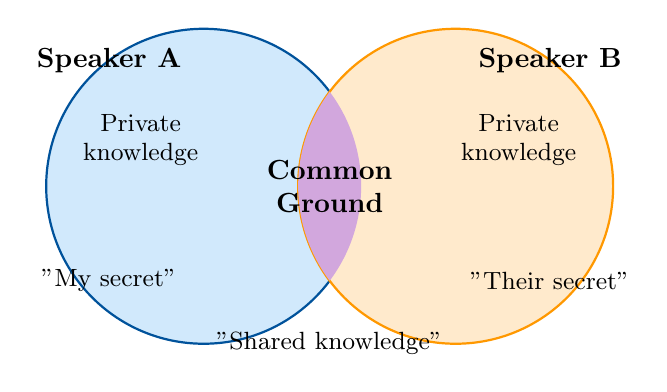
\begin{tikzpicture}[scale=0.8]
            % Speaker A's knowledge
            \draw[fill=lightblue!30, draw=darkblue, thick] (-2,0) circle (2.5cm);
            \node at (-3.5, 2) {\textbf{Speaker A}};
            \node at (-3, 1) {\small Private};
            \node at (-3, 0.5) {\small knowledge};

            % Speaker B's knowledge
            \draw[fill=orange!20, draw=orange, thick] (2,0) circle (2.5cm);
            \node at (3.5, 2) {\textbf{Speaker B}};
            \node at (3, 1) {\small Private};
            \node at (3, 0.5) {\small knowledge};

            % Common ground (intersection)
            \begin{scope}
                \clip (-2,0) circle (2.5cm);
                \fill[purple!40] (2,0) circle (2.5cm);
            \end{scope}

            \node[text width=2cm, align=center] at (0, 0) {\textbf{Common}\\\textbf{Ground}};

            % Labels
            \node at (-3.5, -1.5) {\small "My secret"};
            \node at (3.5, -1.5) {\small "Their secret"};
            \node at (0, -2.5) {\small "Shared knowledge"};
        \end{tikzpicture}
    \end{center}

    \vspace{0.3cm}

    \begin{thinkaboutit}
        Successful communication requires \textbf{tracking} what's in common ground vs. private knowledge!
    \end{thinkaboutit}
\end{frame}

\begin{frame}[shrink=10]{The Grounding Process 🏗️}
\small
    \textbf{How do speakers establish common ground?}

    \vspace{0.3cm}

    \begin{block}{Contribution Model (Clark \& Schaefer, 1989)}
        \begin{enumerate}\setlength{\itemsep}{0pt}
            \item \textbf{Presentation}: Speaker presents utterance
            \item \textbf{Acceptance}: Listener provides evidence of understanding
            \item \textbf{Common ground updated}: Both parties now share this information
        \end{enumerate}
    \end{block}

    \vspace{0.3cm}

    \textbf{Evidence of understanding:}
    \begin{itemize}\setlength{\itemsep}{0pt}
        \item ✅ Continued attention ("uh-huh", "mm-hmm")
        \item ✅ Relevant next contribution
        \item ✅ Acknowledgment ("okay", "right", "I see")
        \item ✅ Demonstration (nodding, following instruction)
        \item ✅ Display (completing the action)
    \end{itemize}
\end{frame}

\begin{frame}[shrink=10]{Grounding Example 💬}
\small
    \begin{block}{Real Conversation Example}
        \textbf{A:} "So we should meet at the \textit{blue} building" \\
        \textbf{B:} "The blue building?" \\
        \textbf{A:} "Yeah, the one next to the library" \\
        \textbf{B:} "Oh! Moore Hall?" \\
        \textbf{A:} "Exactly!" \\
        \textbf{B:} "Got it, Moore Hall at 2pm"
    \end{block}

    \vspace{0.3cm}

    \textbf{What's happening:}
    \begin{enumerate}\setlength{\itemsep}{0pt}
        \item A presents vague reference ("blue building")
        \item B signals confusion/requests clarification
        \item A adds more information
        \item B proposes specific interpretation
        \item A confirms
        \item B demonstrates understanding by repeating full plan
        \item \textbf{Common ground established!} ✅
    \end{enumerate}
\end{frame}

\begin{frame}{Grounding Constraints 🔧}
    \begin{block}{Clark \& Brennan (1991): Grounding Constraints}
        Different communication media impose different constraints on grounding:
    \end{block}

    \vspace{0.3cm}

    \begin{table}
        \small
        \begin{tabular}{lccccc}
            \toprule
            \textbf{Medium} & \textbf{Copresence} & \textbf{Visibility} & \textbf{Audibility} & \textbf{Contemporality} & \textbf{Simultaneity} \\
            \midrule
            Face-to-face & ✅ & ✅ & ✅ & ✅ & ✅ \\
            Video call & ❌ & ✅ & ✅ & ✅ & ✅ \\
            Phone & ❌ & ❌ & ✅ & ✅ & ✅ \\
            Text chat & ❌ & ❌ & ❌ & ✅ & ❌ \\
            Email & ❌ & ❌ & ❌ & ❌ & ❌ \\
            \textbf{Chatbot} & ❌ & ❌ & ❌ & ✅ & ❌ \\
            \bottomrule
        \end{tabular}
    \end{table}

    \vspace{0.3cm}

    \begin{thinkaboutit}
        How do these constraints affect grounding with AI chatbots? What's missing?
    \end{thinkaboutit}
\end{frame}

\begin{frame}{Alignment in Dialogue 🎯}
\small
    \begin{block}{Pickering \& Garrod (2004)}
        \textit{Toward a mechanistic psychology of dialogue}: Speakers automatically \textbf{align} their representations at multiple levels.
    \end{block}

    \vspace{0.3cm}

    \textbf{Levels of alignment:}
    \begin{enumerate}\setlength{\itemsep}{0pt}
        \item \textbf{Lexical}: Using same words
        \item \textbf{Syntactic}: Using same sentence structures
        \item \textbf{Semantic}: Converging on same meanings
        \item \textbf{Phonetic}: Matching pronunciation/accent
        \item \textbf{Situational}: Shared mental model of situation
    \end{enumerate}

    \vspace{0.3cm}

    \begin{alertblock}{Interactive Alignment Model}
        Alignment happens \textbf{automatically} through priming, not conscious effort!
    \end{alertblock}
\end{frame}

\begin{frame}{Lexical Alignment Example 📝}
\small
    \begin{block}{Example: Lexical Entrainment}
        \textbf{A:} "Can you click on the \textit{couch}?" \\
        \textbf{B:} "This \textit{couch}?" \\
        \textbf{A:} "Yes, that \textit{couch}." \\

        \vspace{0.3cm}

        vs. \\

        \vspace{0.3cm}

        \textbf{A:} "Can you click on the \textit{sofa}?" \\
        \textbf{B:} "This \textit{sofa}?" \\
        \textbf{A:} "Yes, that \textit{sofa}."
    \end{block}

    \vspace{0.3cm}

    \textbf{Key findings:}
    \begin{itemize}\setlength{\itemsep}{0pt}
        \item Once speakers agree on a term, they stick with it
        \item This happens even when there are synonyms available
        \item Makes communication more efficient
        \item Builds \textbf{conceptual pacts} (Brennan \& Clark, 1996)
    \end{itemize}
\end{frame}

\begin{frame}{Syntactic Alignment Example 🔄}
    \begin{columns}[T]
        \begin{column}{0.5\textwidth}
            \textbf{Experimenter uses passive:}

            \vspace{0.15cm}

            \textit{"The ball was kicked by the boy"}

            \vspace{0.15cm}

            \textbf{Participant responds:}

            \vspace{0.15cm}

            \textit{"The cake was baked by the chef"} \\
            (Also passive!)
        \end{column}

        \begin{column}{0.5\textwidth}
            \textbf{Experimenter uses active:}

            \vspace{0.15cm}

            \textit{"The boy kicked the ball"}

            \vspace{0.15cm}

            \textbf{Participant responds:}

            \vspace{0.15cm}

            \textit{"The chef baked the cake"} \\
            (Also active!)
        \end{column}
    \end{columns}

    \vspace{0.3cm}

    \begin{thinkaboutit}
        This happens \textbf{unconsciously}! We mimic the syntactic structures we hear.
    \end{thinkaboutit}

    \vspace{0.3cm}

    \textbf{Why does this matter?}
    \begin{itemize}\setlength{\itemsep}{0pt}
        \item Facilitates processing
        \item Signals cooperativeness
        \item Creates smoother conversation flow
    \end{itemize}
\end{frame}

\begin{frame}[shrink=10]{Embodied and Situated Language 🌍}
\small
    \begin{block}{Bisk et al. (2020)}
        \textit{Experience Grounds Language}: Language understanding requires grounding in physical and social experience.
    \end{block}

    \vspace{0.3cm}

    \textbf{The World Scopes framework:}

    \begin{enumerate}\setlength{\itemsep}{0pt}
        \item \textbf{Linguistic}: Text-only (current LLMs)
        \item \textbf{Physical}: Embodied in space/time
        \item \textbf{Perceptual}: Vision, hearing, touch
        \item \textbf{Social}: Multi-agent interaction
        \item \textbf{Cultural}: Norms, values, history
        \item \textbf{Temporal}: Change, events, causation
    \end{enumerate}

    \vspace{0.3cm}

    \begin{alertblock}{The Challenge}
        Most LLMs only have access to \textbf{Scope 1} (linguistic)! Missing 2-6.
    \end{alertblock}
\end{frame}

\begin{frame}[shrink=10]{Why Embodiment Matters 🤖}
\small
    \textbf{Example: "Put the cup on the table"}

    \vspace{0.3cm}

    \begin{columns}[T]
        \begin{column}{0.5\textwidth}
            \textbf{Text-only LLM knows:}
            \begin{itemize}\setlength{\itemsep}{0pt}
                \item ✅ "Cup" is a container
                \item ✅ "Table" is furniture
                \item ✅ "Put" means placement
                \item ✅ "On" is spatial relation
            \end{itemize}
        \end{column}

        \begin{column}{0.5\textwidth}
            \textbf{Embodied agent knows:}
            \begin{itemize}\setlength{\itemsep}{0pt}
                \item ✅ All text-based knowledge
                \item ✅ Cup has weight/fragility
                \item ✅ Table has height/surface
                \item ✅ Gravity pulls cup down
                \item ✅ How to grasp objects
                \item ✅ Navigation required
            \end{itemize}
        \end{column}
    \end{columns}

    \vspace{0.3cm}

    \begin{discussion}
        Can an LLM truly understand "Put the cup on the table" without ever experiencing physical objects, gravity, or spatial relations?
    \end{discussion}
\end{frame}

\section{Language Comprehension and Inference}

\begin{frame}[shrink=10]{Comprehension is Inference 🔍}
\small
    \begin{block}{Graesser et al. (1994)}
        \textit{Constructing Inferences During Narrative Text Comprehension}: Readers actively construct meaning through inference, not passive reception.
    \end{block}

    \vspace{0.3cm}

    \textbf{Types of inferences:}
    \begin{itemize}\setlength{\itemsep}{0pt}
        \item \textbf{Causal antecedent}: What caused this event?
        \item \textbf{Causal consequence}: What will happen next?
        \item \textbf{Goal}: Why is character doing this?
        \item \textbf{Instrument}: How are they doing it?
        \item \textbf{Spatial}: Where is this happening?
        \item \textbf{Emotional}: How does character feel?
    \end{itemize}
\end{frame}

\begin{frame}[shrink=10]{Inference Construction Example 📖}
\small
    \begin{block}{Text}
        "Sarah grabbed her umbrella and rushed out the door."
    \end{block}

    \vspace{0.3cm}

    \textbf{What inferences do you make?}

    \begin{enumerate}\setlength{\itemsep}{0pt}
        \item \textbf{Causal antecedent}: It's raining (or about to rain)
        \item \textbf{Goal}: Sarah wants to stay dry
        \item \textbf{Emotional state}: Sarah is in a hurry / anxious
        \item \textbf{Spatial}: Sarah is leaving her home/building
        \item \textbf{Instrument}: Umbrella will protect from rain
        \item \textbf{Causal consequence}: Sarah will open the umbrella outside
    \end{enumerate}

    \vspace{0.3cm}

    \textbf{None of this is stated explicitly!} Yet you inferred it automatically.

    \vspace{0.3cm}

    \begin{thinkaboutit}
        Do LLMs make these same inferences? How would we know?
    \end{thinkaboutit}
\end{frame}

\begin{frame}[shrink=10]{Embodied Language Processing 👁️}
\small
    \begin{block}{Tanenhaus et al. (1995)}
        \textit{Integration of visual and linguistic information in spoken language comprehension}: Eye movements reveal real-time language processing in visual context.
    \end{block}

    \vspace{0.3cm}

    \textbf{The Visual World Paradigm:}
    \begin{enumerate}\setlength{\itemsep}{0pt}
        \item Show participants visual scene
        \item Play spoken instruction: "Pick up the apple"
        \item Track eye movements
        \item \textbf{Finding}: Eyes move to referent \textit{before} instruction finishes!
    \end{enumerate}

    \vspace{0.3cm}

    \textbf{Key insights:}
    \begin{itemize}\setlength{\itemsep}{0pt}
        \item Language processing is \textbf{incremental} (word-by-word)
        \item Visual context \textbf{immediately} influences interpretation
        \item Language and vision are \textbf{tightly coupled}
        \item Processing is \textbf{predictive}, not just reactive
    \end{itemize}
\end{frame}

\begin{frame}[shrink=10]{Referential Ambiguity Resolution 🎯}
    \textbf{Example scenario:}

    \vspace{0.3cm}

    Visual scene contains:
    \begin{itemize}\setlength{\itemsep}{0pt}
        \item Large red apple
        \item Small red apple
        \item Large green apple
        \item Red ball
    \end{itemize}

    \vspace{0.3cm}

    \textbf{Instruction}: "Pick up the small apple"

    \vspace{0.3cm}

    \begin{columns}[T]
        \begin{column}{0.5\textwidth}
            \textbf{Human processing:}
            \begin{enumerate}\setlength{\itemsep}{0pt}
                \item Hears "Pick up the..."
                \item Eyes scan objects
                \item Hears "small..."
                \item Eyes fixate small apple
                \item Before "apple" finishes!
            \end{enumerate}
        \end{column}

        \begin{column}{0.5\textwidth}
            \textbf{LLM processing:}
            \begin{itemize}\setlength{\itemsep}{0pt}
                \item ❌ No visual scene
                \item ❌ No eye movements
                \item ❌ No incremental visual search
                \item ✅ Can imagine scenario
                \item ❓ Is imagination enough?
            \end{itemize}
        \end{column}
    \end{columns}
\end{frame}

\section{Thought Trajectories}

\begin{frame}{Mental Trajectories During Comprehension 🧠}
\small
    \begin{block}{Heusser et al. (2021)}
        \textit{Geometric models reveal behavioral and neural signatures of transforming experiences into memories}: Thoughts follow trajectories through mental space during narrative comprehension.
    \end{block}

    \vspace{0.3cm}

    \textbf{Key idea:}
    \begin{itemize}\setlength{\itemsep}{0pt}
        \item Mental representations can be modeled as points in high-dimensional space
        \item During comprehension, thoughts "move" through this space
        \item Can track these trajectories using fMRI + computational models
        \item Trajectories predict memory, comprehension, and engagement
    \end{itemize}

    \vspace{0.3cm}

    \begin{alertblock}{Connection to LLMs}
        Transformer hidden states also form trajectories! Can we compare human and model thought trajectories?
    \end{alertblock}
\end{frame}

\begin{frame}[shrink=5]{Visualizing Thought Trajectories 📊}
    \begin{center}
        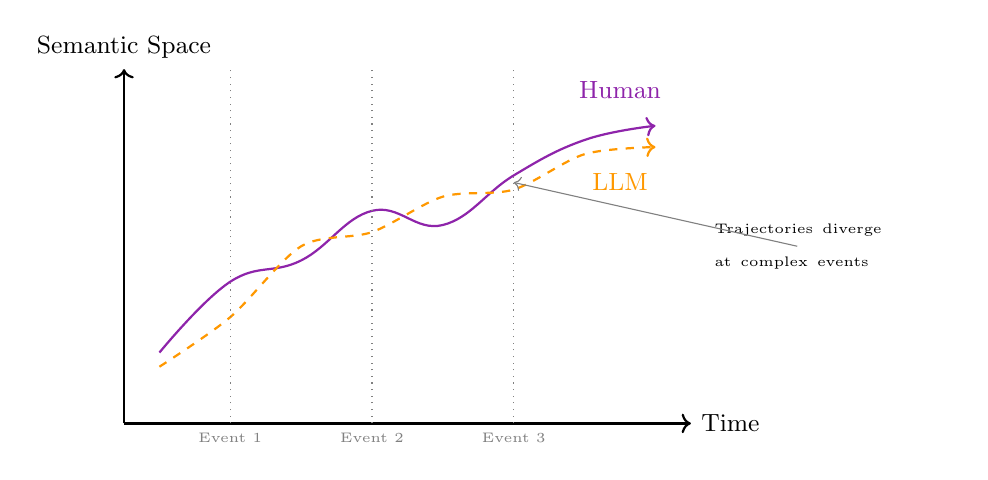
\begin{tikzpicture}[scale=0.9]
            % Axes
            \draw[->, thick] (0,0) -- (8,0) node[right] {\small Time};
            \draw[->, thick] (0,0) -- (0,5) node[above] {\small Semantic Space};

            % Human trajectory (smooth, organic)
            \draw[thick, purple, ->]
                plot[smooth, tension=0.7] coordinates {
                    (0.5,1) (1.5,2) (2.5,2.3) (3.5,3) (4.5,2.8) (5.5,3.5) (6.5,4) (7.5,4.2)
                };
            \node[purple] at (7, 4.7) {\small Human};

            % LLM trajectory (more mechanical)
            \draw[thick, orange, dashed, ->]
                plot[smooth, tension=0.5] coordinates {
                    (0.5,0.8) (1.5,1.5) (2.5,2.5) (3.5,2.7) (4.5,3.2) (5.5,3.3) (6.5,3.8) (7.5,3.9)
                };
            \node[orange] at (7, 3.4) {\small LLM};

            % Event markers
            \foreach \x/\label in {1.5/Event 1, 3.5/Event 2, 5.5/Event 3} {
                \draw[gray, dotted] (\x,0) -- (\x,5);
                \node[gray, below] at (\x,0) {\tiny \label};
            }

            % Annotation
            \node[text width=3cm, align=left] at (10, 2.5) {
                \tiny Trajectories diverge\\
                \tiny at complex events
            };
            \draw[->, gray] (9.5, 2.5) -- (5.5, 3.4);
        \end{tikzpicture}
    \end{center}

    \vspace{0.3cm}

    \textbf{Questions to explore:}
    \begin{itemize}\setlength{\itemsep}{0pt}
        \item Do LLM trajectories match human trajectories?
        \item Where do they diverge?
        \item What does this tell us about understanding?
    \end{itemize}
\end{frame}

\begin{frame}{Context-Dependent Representations 🔄}
    \begin{block}{Manning (2021)}
        \textit{Human Language Understanding \& Reasoning}: Contextual representations in transformers show similarities to human language processing.
    \end{block}

    \vspace{0.3cm}

    \textbf{Example: Word "bank"}

    \begin{columns}[T]
        \begin{column}{0.5\textwidth}
            \textbf{Context 1:}

            \textit{"I deposited money at the \underline{bank}"}

            \vspace{0.15cm}

            Representation: \\
            $\vec{v}_{\text{bank}} \approx$ [financial, institution, money, ...]
        \end{column}

        \begin{column}{0.5\textwidth}
            \textbf{Context 2:}

            \textit{"We sat by the river \underline{bank}"}

            \vspace{0.15cm}

            Representation: \\
            $\vec{v}_{\text{bank}} \approx$ [shore, edge, water, ...]
        \end{column}
    \end{columns}

    \vspace{0.3cm}

    \textbf{Both humans and transformers:}
    \begin{itemize}\setlength{\itemsep}{0pt}
        \item ✅ Create context-dependent representations
        \item ✅ Resolve ambiguity using surrounding words
        \item ✅ Update interpretations incrementally
    \end{itemize}
\end{frame}

\section{Positional Coding, Context, and Memory}

\begin{frame}[shrink=10]{The Problem of Position 📍}
    \textbf{Challenge for transformers:}

    \vspace{0.3cm}

    \begin{alertblock}{Problem}
        Transformers process all tokens \textbf{in parallel}—they don't inherently know word order!
    \end{alertblock}

    \vspace{0.3cm}

    \begin{columns}[T]
        \begin{column}{0.5\textwidth}
            \textbf{These are different:}
            \begin{itemize}\setlength{\itemsep}{0pt}
                \item "Dog bites man"
                \item "Man bites dog"
            \end{itemize}

            Same words, \textbf{different order}, different meaning!
        \end{column}

        \begin{column}{0.5\textwidth}
            \textbf{Without position info:}
            \begin{itemize}\setlength{\itemsep}{0pt}
                \item Transformer sees: \{dog, bites, man\}
                \item Can't distinguish the two!
                \item \textbf{Solution}: Add positional encoding
            \end{itemize}
        \end{column}
    \end{columns}
\end{frame}

\begin{frame}{Positional Encoding in Transformers 🔢}
\small
    \begin{block}{Vaswani et al. (2017) - "Attention is All You Need"}
        Use sinusoidal functions to encode position:
    \end{block}

    \vspace{0.3cm}

    $$PE_{(pos, 2i)} = \sin\left(\frac{pos}{10000^{2i/d}}\right)$$
    $$PE_{(pos, 2i+1)} = \cos\left(\frac{pos}{10000^{2i/d}}\right)$$

    \vspace{0.3cm}

    \textbf{Why this works:}
    \begin{itemize}\setlength{\itemsep}{0pt}
        \item Each position gets a unique pattern
        \item Relative positions have consistent relationships
        \item Model can learn to attend to relative distances
        \item Generalizes to longer sequences than seen in training
    \end{itemize}

    \vspace{0.3cm}

    \begin{thinkaboutit}
        This is very different from how humans track position in language! We use temporal order naturally.
    \end{thinkaboutit}
\end{frame}

\begin{frame}[shrink=5]{Visualizing Positional Encodings 📈}
    \begin{center}
        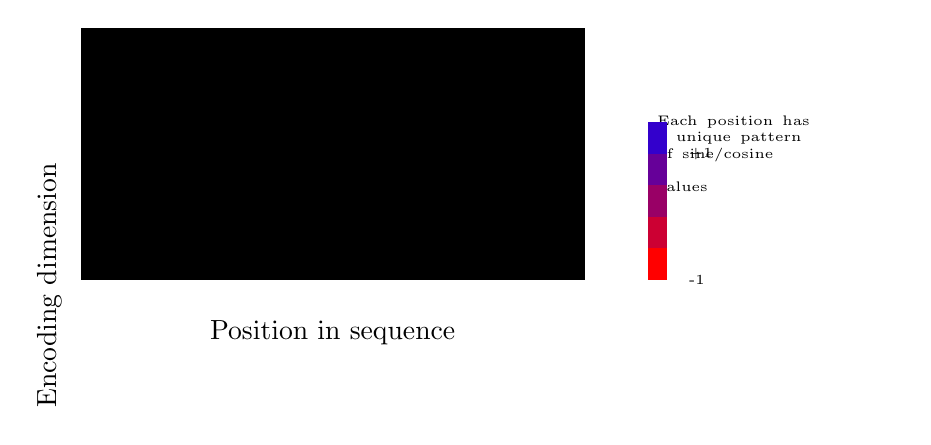
\begin{tikzpicture}[scale=0.8]
            % Draw heatmap-style visualization
            \foreach \pos in {0,...,9} {
                \foreach \dim in {0,...,7} {
                    % Calculate approximate value (simplified for visualization)
                    \pgfmathsetmacro{\val}{sin(\pos * 180 / (2 + \dim))}
                    \pgfmathsetmacro{\color}{50 + 50*\val}
                    \fill[blue!\color!red] (\pos*0.8, \dim*0.5) rectangle +(0.8, 0.5);
                }
            }

            % Labels
            \node[below] at (4, -0.5) {Position in sequence};
            \node[left, rotate=90] at (-0.5, 2) {Encoding dimension};

            % Add legend
            \node[right, text width=3cm] at (9, 2) {
                \tiny Each position has\\
                \tiny a unique pattern\\
                \tiny of sine/cosine\\
                \tiny values
            };

            % Color scale
            \foreach \i in {0,...,4} {
                \pgfmathsetmacro{\c}{20*\i}
                \fill[blue!\c!red] (9, \i*0.5) rectangle +(0.3, 0.5);
            }
            \node[right] at (9.5, 0) {\tiny -1};
            \node[right] at (9.5, 2) {\tiny +1};
        \end{tikzpicture}
    \end{center}

    \vspace{0.3cm}

    Each column is a position (0-9), each row is a dimension of the encoding
\end{frame}

\begin{frame}[shrink=10]{Context and Memory in Transformers 🧠}
\small
    \begin{block}{Manning (2023)}
        \textit{Positional Information in Transformers}: Position encoding enables transformers to maintain context and sequence information.
    \end{block}

    \vspace{0.3cm}

    \textbf{Types of context:}

    \begin{enumerate}\setlength{\itemsep}{0pt}
        \item \textbf{Local context}: Nearby words (via attention)
        \item \textbf{Long-range dependencies}: Distant words (via attention)
        \item \textbf{Positional context}: Where in sequence (via PE)
        \item \textbf{Semantic context}: Topic/meaning (via embeddings)
    \end{enumerate}

    \vspace{0.3cm}

    \textbf{Memory limitations:}
    \begin{itemize}\setlength{\itemsep}{0pt}
        \item Context window: typically 2K-100K tokens
        \item Beyond this, model "forgets" earlier content
        \item Trade-off: longer context = more computation
    \end{itemize}
\end{frame}

\begin{frame}[shrink=10]{Human vs. Transformer Memory 🔄}
\small
    \begin{columns}[T]
        \begin{column}{0.5\textwidth}
            \textbf{Human conversation memory:}
            \begin{itemize}\setlength{\itemsep}{0pt}
                \item Episodic memory of past conversations
                \item Semantic knowledge from experience
                \item Working memory (7±2 items)
                \item Long-term memory (lifetime)
                \item Gist-based storage
                \item Reconstructive retrieval
                \item Context-dependent recall
            \end{itemize}
        \end{column}

        \begin{column}{0.5\textwidth}
            \textbf{Transformer "memory":}
            \begin{itemize}\setlength{\itemsep}{0pt}
                \item Parameters (training data)
                \item Context window (recent tokens)
                \item No episodic memory
                \item No true long-term memory
                \item Exact token storage (in window)
                \item Perfect recall (within window)
                \item Hard cutoff at context limit
            \end{itemize}
        \end{column}
    \end{columns}

    \vspace{0.3cm}

    \begin{discussion}
        If a chatbot can't remember our previous conversation, can it truly have a "relationship" with us?
    \end{discussion}
\end{frame}

\section{Human vs. Model Conversation}

\begin{frame}{Comparing Human and Chatbot Conversations 💬🤖}
    \textbf{Key dimensions of comparison:}

    \vspace{0.3cm}

    \begin{table}
        \small
        \begin{tabular}{lcc}
            \toprule
            \textbf{Feature} & \textbf{Human} & \textbf{Chatbot} \\
            \midrule
            Common ground building & ✅ & Simulated \\
            Grounding process & ✅ & Limited \\
            Alignment & ✅ & Partial \\
            Embodied understanding & ✅ & ❌ \\
            Pragmatic reasoning & ✅ & Improving \\
            Memory of conversation & ✅ & Window-based \\
            Emotional understanding & ✅ & Simulated \\
            Goal-directed action & ✅ & Task-dependent \\
            Social awareness & ✅ & Limited \\
            Contextual adaptation & ✅ & ✅ \\
            \bottomrule
        \end{tabular}
    \end{table}
\end{frame}

\begin{frame}[shrink=10]{Can Language Models Have Common Ground? 🤔}
\small
    \begin{discussion}
        Can a language model \textit{truly} establish common ground with a user?
    \end{discussion}

    \vspace{0.3cm}

    \begin{columns}[T]
        \begin{column}{0.5\textwidth}
            \textbf{Arguments for "Yes":}
            \begin{itemize}\setlength{\itemsep}{0pt}
                \item Can track conversation history
                \item Can make inferences about user knowledge
                \item Can adapt language to user
                \item Can reference shared context
                \item Can align representations
            \end{itemize}
        \end{column}

        \begin{column}{0.5\textwidth}
            \textbf{Arguments for "No":}
            \begin{itemize}\setlength{\itemsep}{0pt}
                \item No persistent memory across sessions
                \item No embodied shared experience
                \item No genuine beliefs/knowledge
                \item No personal history
                \item No cultural grounding
                \item Simulates vs. experiences
            \end{itemize}
        \end{column}
    \end{columns}

    \vspace{0.3cm}

    \begin{thinkaboutit}
        Perhaps the question is: Does it matter? If interaction feels collaborative, is that enough?
    \end{thinkaboutit}
\end{frame}

\begin{frame}[shrink=10]{Pragmatic Reasoning Example 🧩}
\small
    \begin{block}{Scenario}
        \textbf{User:} "I'm looking for a good Italian restaurant" \\
        \textbf{Chatbot:} "I'd recommend Bella Vista. Would you like the address?"
    \end{block}

    \vspace{0.3cm}

    \textbf{What pragmatic inferences is chatbot making?}

    \begin{enumerate}\setlength{\itemsep}{0pt}
        \item User wants to \textit{go} to restaurant (not just learn about it)
        \item User is likely nearby / asking about local options
        \item User wants recommendation (not exhaustive list)
        \item Offering address implies user will visit
        \item "Good" implies quality, not just any restaurant
    \end{enumerate}

    \vspace{0.3cm}

    \textbf{But chatbot doesn't actually know:}
    \begin{itemize}\setlength{\itemsep}{0pt}
        \item User's location
        \item User's food preferences
        \item User's budget
        \item Time/date of desired visit
    \end{itemize}
\end{frame}

\begin{frame}[fragile]{Interactive Pragmatic Reasoning 💡}
\small
    \begin{block}{Better Grounding Strategy}
        \textbf{User:} "I'm looking for a good Italian restaurant" \\
        \textbf{Chatbot:} "I'd be happy to help! A few questions:" \\
        \textbf{Chatbot:} "- What city are you in?" \\
        \textbf{Chatbot:} "- What's your price range?" \\
        \textbf{Chatbot:} "- Any dietary restrictions?"
    \end{block}

    \vspace{0.3cm}

    \textbf{This mirrors human conversation!}

    \begin{itemize}\setlength{\itemsep}{0pt}
        \item Humans ask clarifying questions
        \item Build common ground iteratively
        \item Don't assume unstated information
        \item Confirm understanding before proceeding
    \end{itemize}

    \vspace{0.3cm}

    \begin{thinkaboutit}
        Modern chatbots are getting better at this, but still often assume too much or ask too little.
    \end{thinkaboutit}
\end{frame}

\section{Demo: ConvoKit}

\begin{frame}[shrink=10]{ConvoKit: Analyzing Real Conversations 🔬}
\small
    \begin{block}{What is ConvoKit?}
        ConvoKit is a Python toolkit for analyzing conversations, created by researchers at Cornell.
    \end{block}

    \vspace{0.3cm}

    \textbf{Features:}
    \begin{itemize}\setlength{\itemsep}{0pt}
        \item Pre-loaded conversation datasets (Reddit, Wikipedia, Supreme Court, etc.)
        \item Tools for analyzing conversational dynamics
        \item Coordination measures
        \item Politeness analysis
        \item Question types
        \item Conversational structure
    \end{itemize}

    \vspace{0.3cm}

    \textbf{Why useful for this course:}
    \begin{itemize}\setlength{\itemsep}{0pt}
        \item Study real conversational patterns
        \item Compare human vs. bot conversations
        \item Measure alignment, grounding, pragmatics
        \item Build better conversational agents
    \end{itemize}
\end{frame}

\begin{frame}[fragile]{ConvoKit: Installation and Setup 🛠️}
    \begin{lstlisting}
# Install ConvoKit
!pip install convokit

# Import library
import convokit
from convokit import Corpus, download

# Load a pre-built corpus
corpus = Corpus(filename=download("reddit-corpus-small"))

# Explore the corpus
print(f"Number of conversations: {len(corpus.conversations)}")
print(f"Number of utterances: {len(corpus.utterances)}")
print(f"Number of speakers: {len(corpus.speakers)}")
    \end{lstlisting}

    \vspace{0.3cm}

    \textbf{Available corpora:}
    \begin{itemize}\setlength{\itemsep}{0pt}
        \item Reddit conversations
        \item Wikipedia talk pages
        \item Movie dialogs
        \item Supreme Court oral arguments
        \item ... and more!
    \end{itemize}
\end{frame}

\begin{frame}[fragile]{ConvoKit: Analyzing Coordination 🤝}
    \textbf{Linguistic coordination}: Do speakers align their language?

    \begin{lstlisting}
from convokit import Coordination

# Initialize coordination analyzer
coord = Coordination()

# Compute coordination scores
corpus = coord.fit_transform(corpus)

# Get coordination between two speakers
for convo in corpus.iter_conversations():
    speakers = list(convo.get_speaker_ids())
    if len(speakers) >= 2:
        score = coord.score(corpus, speaker1=speakers[0],
                           speaker2=speakers[1])
        print(f"Coordination score: {score}")
        break
    \end{lstlisting}

    \vspace{0.3cm}

    \textbf{What this measures:}
    \begin{itemize}\setlength{\itemsep}{0pt}
        \item Lexical alignment (using same words)
        \item Function word coordination
        \item Syntactic priming
    \end{itemize}
\end{frame}

\begin{frame}[fragile]{ConvoKit: Politeness Analysis 🎩}
    \begin{lstlisting}
from convokit import PolitenessStrategies

# Initialize politeness analyzer
ps = PolitenessStrategies()

# Analyze politeness in utterances
corpus = ps.fit_transform(corpus,
                          markers=True)

# Check politeness of specific utterance
for utterance in corpus.iter_utterances():
    if utterance.meta.get('politeness_strategies'):
        strategies = utterance.meta['politeness_strategies']
        print(f"Text: {utterance.text}")
        print(f"Politeness markers: {strategies}")
        break
    \end{lstlisting}

    \vspace{0.3cm}

    \textbf{Politeness strategies detected:}
    \begin{itemize}\setlength{\itemsep}{0pt}
        \item Please, gratitude
        \item Hedges, deference
        \item Indirect requests
        \item Formal titles
    \end{itemize}
\end{frame}

\begin{frame}[fragile]{ConvoKit: Question Analysis ❓}
    \begin{lstlisting}
from convokit import QuestionTypology

# Initialize question analyzer
qt = QuestionTypology()

# Analyze questions in conversations
corpus = qt.fit_transform(corpus)

# Examine question types
for utterance in corpus.iter_utterances():
    if utterance.meta.get('question_type'):
        qtype = utterance.meta['question_type']
        print(f"Question: {utterance.text}")
        print(f"Type: {qtype}")
        print(f"Awaits response: {utterance.meta.get('awaits_response')}")
        print()
    \end{lstlisting}

    \vspace{0.3cm}

    \textbf{Question types:}
    \begin{itemize}\setlength{\itemsep}{0pt}
        \item Rhetorical vs. information-seeking
        \item Yes/no vs. open-ended
        \item Clarification requests
    \end{itemize}
\end{frame}

\begin{frame}[fragile]{ConvoKit: Conversation Structure 🏗️}
    \begin{lstlisting}
# Analyze turn-taking and threading
for convo in corpus.iter_conversations():
    print(f"Conversation ID: {convo.id}")
    print(f"Number of turns: {len(list(convo.iter_utterances()))}")

    # Get conversation tree structure
    root = convo.get_root_utterance()
    print(f"Root: {root.text[:50]}...")

    # Traverse conversation tree
    for reply in root.iter_children():
        print(f"  Reply: {reply.text[:50]}...")
        for nested_reply in reply.iter_children():
            print(f"    Nested: {nested_reply.text[:50]}...")

    break  # Just show first conversation
    \end{lstlisting}

    \vspace{0.3cm}

    \textbf{Understanding structure:}
    \begin{itemize}\setlength{\itemsep}{0pt}
        \item Threading (nested replies)
        \item Turn-taking patterns
        \item Response times
    \end{itemize}
\end{frame}

\begin{frame}{ConvoKit Example: Reddit Analysis 📊}
\small
    \textbf{Real example from Reddit data:}

    \vspace{0.3cm}

    \begin{block}{Conversation}
        \textbf{User A:} "Does anyone know how to fix a squeaky door?" \\
        \textbf{User B:} "WD-40 usually works" \\
        \textbf{User A:} "Thanks! I'll try that" \\
        \textbf{User C:} "Actually, use silicone spray, not WD-40" \\
        \textbf{User A:} "Oh, why's that?" \\
        \textbf{User C:} "WD-40 attracts dust. Silicone is better for hinges"
    \end{block}

    \vspace{0.3cm}

    \textbf{ConvoKit analysis reveals:}
    \begin{itemize}\setlength{\itemsep}{0pt}
        \item User A uses more politeness markers ("Thanks!", question marks)
        \item User C coordinates with User A (both use "WD-40")
        \item Thread structure: A $\rightarrow$ B, A $\rightarrow$ C (parallel responses)
        \item Question types: information-seeking (A), clarification (A)
    \end{itemize}
\end{frame}

\begin{frame}[shrink=10]{Using ConvoKit for Chatbot Evaluation 🤖}
    \textbf{How to use ConvoKit to evaluate your chatbot:}

    \vspace{0.3cm}

    \begin{enumerate}\setlength{\itemsep}{0pt}
        \item \textbf{Collect conversations} between users and your chatbot
        \item \textbf{Convert to ConvoKit format}
        \item \textbf{Compare to human-human conversations:}
        \begin{itemize}\setlength{\itemsep}{0pt}
            \item Is chatbot coordinating with users?
            \item Does it use appropriate politeness?
            \item Does it ask good questions?
            \item Does it provide relevant responses?
        \end{itemize}
        \item \textbf{Identify weaknesses}
        \item \textbf{Improve your model}
    \end{enumerate}

    \vspace{0.3cm}

    \begin{alertblock}{Assignment Idea}
        You could use ConvoKit to analyze your ELIZA chatbot conversations and compare to real therapy session transcripts!
    \end{alertblock}
\end{frame}

\begin{frame}[fragile]{ConvoKit: Creating Your Own Corpus 📝}
    \begin{lstlisting}
from convokit import Corpus, Speaker, Utterance

# Create speakers
alice = Speaker(id="alice", meta={"name": "Alice"})
bob = Speaker(id="bob", meta={"name": "Bob"})

# Create utterances
utterances = [
    Utterance(id="1", speaker=alice, text="Hi Bob!",
              timestamp=0),
    Utterance(id="2", speaker=bob, text="Hey Alice!",
              reply_to="1", timestamp=1),
    Utterance(id="3", speaker=alice, text="How are you?",
              reply_to="2", timestamp=2),
]

# Create corpus
my_corpus = Corpus(utterances=utterances)

# Now you can analyze it with ConvoKit tools!
    \end{lstlisting}

    \vspace{0.3cm}

    \textbf{Use case:} Analyze your own chatbot conversations!
\end{frame}

\section{Discussion and Wrap-up}

\begin{frame}{Discussion: Grounding in Human-AI Interaction 🤔}
\small
    \begin{discussion}
        Consider these questions:

        \begin{enumerate}\setlength{\itemsep}{0pt}
            \item Do you engage in grounding when talking to ChatGPT or other LLMs?
            \item Do you adjust your language when the model doesn't understand?
            \item Does the model adjust to \textit{you}?
            \item Do you feel like you're building common ground?
            \item What's missing from AI conversations compared to human ones?
        \end{enumerate}
    \end{discussion}

    \vspace{0.3cm}

    \begin{thinkaboutit}
        Think about your most recent conversation with an AI. Did you treat it like a person, a tool, or something in between?
    \end{thinkaboutit}
\end{frame}

\begin{frame}{The Turing Test Revisited 🎭}
\small
    \begin{block}{Turing (1950): "Can Machines Think?"}
        Instead of defining thinking, ask: Can a machine's conversation be distinguished from a human's?
    \end{block}

    \vspace{0.3cm}

    \textbf{Modern perspective:}
    \begin{itemize}\setlength{\itemsep}{0pt}
        \item Many chatbots can "pass" brief Turing tests
        \item But: This tests \textit{imitation}, not understanding
        \item Pragmatics, grounding, and common ground reveal differences
        \item Longer conversations expose limitations
    \end{itemize}

    \vspace{0.3cm}

    \begin{alertblock}{Important Distinction}
        \textbf{Appearing to understand} $\neq$ \textbf{Actually understanding}

        But: Is there a meaningful difference if the \textit{functional behavior} is identical?
    \end{alertblock}
\end{frame}

\begin{frame}[shrink=10]{Future Directions 🔮}
    \textbf{What would make LLM conversations more human-like?}

    \vspace{0.3cm}

    \begin{enumerate}\setlength{\itemsep}{0pt}
        \item \textbf{Better grounding mechanisms}
        \begin{itemize}\setlength{\itemsep}{0pt}
            \item Explicit confirmation strategies
            \item Clarification requests
            \item Incremental understanding updates
        \end{itemize}

        \item \textbf{Embodied and situated models}
        \begin{itemize}\setlength{\itemsep}{0pt}
            \item Multimodal understanding (vision + language)
            \item Physical world knowledge
            \item Temporal and causal reasoning
        \end{itemize}

        \item \textbf{Persistent memory and personalization}
        \begin{itemize}\setlength{\itemsep}{0pt}
            \item Long-term conversation history
            \item User models and preferences
            \item Relationship building
        \end{itemize}

        \item \textbf{Social and cultural awareness}
        \begin{itemize}\setlength{\itemsep}{0pt}
            \item Pragmatic norms
            \item Cultural context
            \item Emotional intelligence
        \end{itemize}
    \end{enumerate}
\end{frame}

\begin{frame}[shrink=10]{Key Takeaways 🔑}
    \begin{enumerate}\setlength{\itemsep}{0pt}
        \item \textbf{Language is for action}, not just description

        \item \textbf{Pragmatics} is essential: meaning depends on context

        \item \textbf{Common ground} and \textbf{grounding} are fundamental to conversation

        \item \textbf{Alignment} happens automatically in human dialogue

        \item \textbf{Embodied understanding} provides grounding that text-only models lack

        \item \textbf{Comprehension involves active inference}, not passive reception

        \item \textbf{Thought trajectories} can be modeled and compared across humans/LLMs

        \item \textbf{Positional encoding} enables transformers to track sequence order

        \item \textbf{LLMs simulate} many conversational abilities, but with important limitations

        \item \textbf{Tools like ConvoKit} let us analyze and improve conversational systems
    \end{enumerate}
\end{frame}

\begin{frame}{Readings for This Week 📖}
\small
    \begin{block}{Required Readings}
        \begin{enumerate}\setlength{\itemsep}{0pt}
            \item \textbf{Clark \& Brennan (1991)}: Grounding in Communication \\
            \href{https://www.sciencedirect.com/science/article/pii/B9780080507378500167}{[Link]}

            \item \textbf{Pickering \& Garrod (2004)}: Toward a mechanistic psychology of dialogue \\
            \href{https://www.cambridge.org/core/journals/behavioral-and-brain-sciences/article/toward-a-mechanistic-psychology-of-dialogue/D9C9E72F9DDCB6494A0F156A97DCC6C7}{[Link]}

            \item \textbf{Bisk et al. (2020)}: Experience Grounds Language \\
            \href{https://arxiv.org/abs/2004.10151}{[ArXiv]}

            \item \textbf{Graesser et al. (1994)}: Constructing Inferences During Narrative Text Comprehension \\
            \href{https://psycnet.apa.org/record/1994-97967-001}{[Link]}

            \item \textbf{Tanenhaus et al. (1995)}: Integration of visual and linguistic information \\
            \href{https://www.science.org/doi/10.1126/science.7777863}{[Science]}
        \end{enumerate}
    \end{block}
\end{frame}

\begin{frame}{Readings for This Week (continued) 📖}
\small
    \begin{block}{Required Readings (continued)}
        \begin{enumerate}\setlength{\itemsep}{0pt}
            \setcounter{enumi}{5}
            \item \textbf{Heusser et al. (2021)}: Geometric models reveal behavioral and neural signatures of transforming experiences into memories \\
            \href{https://www.nature.com/articles/s41562-021-01051-6}{[Nature Human Behaviour]}

            \item \textbf{Manning (2021)}: Human Language Understanding \& Reasoning \\
            \href{https://www.cambridge.org/core/journals/natural-language-engineering}{[Link]}

            \item \textbf{Manning (2023)}: Positional Information in Transformers \\
            \href{https://arxiv.org/abs/2305.16642}{[ArXiv]}
        \end{enumerate}
    \end{block}

    \vspace{0.3cm}

    \begin{block}{Optional: ConvoKit}
        \item \textbf{ConvoKit Documentation}: \href{https://convokit.cornell.edu/}{https://convokit.cornell.edu/}
    \end{block}
\end{frame}

\begin{frame}[shrink=10]{Next Week Preview 🔮}
\small
    \begin{block}{Week 8: Neural Foundations of Language Models}
        We'll explore:
        \begin{itemize}\setlength{\itemsep}{0pt}
            \item Neural network basics
            \item Word embeddings (Word2Vec, GloVe)
            \item Recurrent neural networks (RNNs, LSTMs)
            \item Sequence-to-sequence models
            \item Attention mechanisms
        \end{itemize}
    \end{block}

    \vspace{0.3cm}

    \textbf{Preparation:}
    \begin{itemize}\setlength{\itemsep}{0pt}
        \item Review linear algebra (vectors, matrices, dot products)
        \item Python/NumPy basics
        \item Start thinking about final project ideas!
    \end{itemize}
\end{frame}

\begin{frame}{Questions and Discussion 💬}
    \begin{center}
        \Large{Let's discuss!}

        \vspace{0.5cm}

        \textbf{Contact Information:}

        📧 jeremy@dartmouth.edu

        💬 Discord: \href{https://discord.gg/sftEk9Ygdw}{https://discord.gg/sftEk9Ygdw}

        🏢 Office Hours: By appointment (Moore Hall 349)

        \vspace{0.5cm}

        \textbf{Try ConvoKit this week!} 🔬

        \vspace{0.3cm}

        \large{See you next week! 🚀}
    \end{center}
\end{frame}

\end{document}
